\documentclass[UTF8,zihao=5,scheme=chinese]{ctexart}

\newcommand{\UniversityName}{武汉大学}
\newcommand{\CollegeName}{计算机学院}
\newcommand{\MajorName}{计算机科学与技术（雷军班）}
\newcommand{\CourseName}{自动驾驶技术}
\newcommand{\ReportTitle}{自动驾驶技术第一次实验报告}
\newcommand{\ReportSubtitle}{nuScenes 数据处理与 YOLO 视觉目标检测}
\newcommand{\StudentName}{尹玉文东}
\newcommand{\StudentID}{2024302131025}
\newcommand{\InstructorName}{张红娟}
\newcommand{\CompletionDate}{2026年9月23日}
\usepackage{../template/course-report}

\begin{document}

\makecoursecover
\tableofcontents
\clearpage

\section{实验概述}

这次实践从 nuScenes 数据读取开始。我用 DevKit 查看相机图像、点云和三维标注，再把点云
与目标框投影到前视图像。课程提供了转换好的 YOLO 数据，我检查标签后，在 One-North 上
训练并测试了 YOLO11n，最后用同一模型测试另外三个地区。
文中脚本路径以随报告发送的源代码根目录为起点。

\section{实验环境与数据准备}

\subsection{软硬件环境}

实验在 WSL2 Ubuntu 环境下完成，使用 uv 管理依赖。PyTorch 能够识别 RTX 4060。

\begin{table}[htbp]
  \centering
  \caption{主要实验环境}
  \label{tab:environment}
  \begin{tabular}{ll}
    \toprule
    项目 & 配置 \\
    \midrule
    操作环境 & WSL2 Ubuntu \\
    GPU & NVIDIA GeForce RTX 4060（8 GB） \\
    NVIDIA 驱动 & 591.86 \\
    Python & 3.12.14 \\
    PyTorch & 2.14.0 + CUDA 13.0 \\
    cuDNN & 9.24 \\
    nuScenes-devkit & 1.2.0 \\
    Ultralytics & 8.4.152 \\
    \bottomrule
  \end{tabular}
\end{table}

\subsection{数据准备与目录规划}

nuScenes 数据保存在机械硬盘，项目通过 \texttt{data} 软链接访问。目录如下：

\begin{minted}[linenos=false]{text}
data/nuscenes/
  maps/
  samples/
    CAM_FRONT/        CAM_BACK/
    CAM_FRONT_LEFT/   CAM_BACK_LEFT/
    CAM_FRONT_RIGHT/  CAM_BACK_RIGHT/
    LIDAR_TOP/
    RADAR_FRONT/      RADAR_FRONT_LEFT/
    RADAR_FRONT_RIGHT/
    RADAR_BACK_LEFT/  RADAR_BACK_RIGHT/
  v1.0-trainval/
\end{minted}

我统计了传感器文件：六路相机和 LIDAR\_TOP 各有 40,157 个，五路 Radar 各有约 34,147 个
关键帧文件。DevKit 读出了 850 个 scene、34,149 个 sample 和 1,166,187 条标注。

老师提供的二维检测数据按四个地区组织，规模见表~\ref{tab:yolo-data}。我检查了图像与
标签是否对应，以及类别编号和坐标是否有效。训练使用 One-North。

\begin{table}[htbp]
  \centering
  \caption{四个地区的 YOLO 数据规模}
  \label{tab:yolo-data}
  \begin{tabular}{lrrrr}
    \toprule
    地区 & Train & Val & Test & 合计 \\
    \midrule
    Boston Seaport & 9,420 & 1,402 & 2,709 & 13,531 \\
    Holland Village & 365 & 56 & 88 & 509 \\
    One-North & 3,634 & 461 & 1,015 & 5,110 \\
    Queenstown & 1,661 & 205 & 486 & 2,352 \\
    \midrule
    合计 & 15,080 & 2,124 & 4,298 & 21,502 \\
    \bottomrule
  \end{tabular}
\end{table}

\section{nuScenes 数据集格式与组织}

\subsection{真实文件与元数据表}

nuScenes~\cite{nuscenes} 将数据分开保存。\texttt{samples} 存放图像和点云文件，
\texttt{v1.0-trainval} 中的 JSON 表记录文件关联，\texttt{maps} 保存地图图像。

本次用到的数据表见表~\ref{tab:nuscenes-tables}。各表通过 token 关联。

\begin{table}[htbp]
  \centering
  \caption{实验涉及的 nuScenes 核心数据表}
  \label{tab:nuscenes-tables}
  \begin{tabularx}{\linewidth}{lX}
    \toprule
    数据表 & 作用 \\
    \midrule
    \texttt{scene.json} & 记录连续驾驶片段及其首尾 sample token \\
    \texttt{sample.json} & 记录关键时刻及前后 sample、传感器数据和标注 token \\
    \texttt{sample\_data.json} & 记录传感器文件名、时间戳、标定和车辆位姿 token \\
    \texttt{calibrated\_sensor.json} & 保存传感器相对车辆坐标系的外参以及相机内参 \\
    \texttt{ego\_pose.json} & 保存采集时刻车辆在全局坐标系中的位置和姿态 \\
    \texttt{sample\_annotation.json} & 保存目标类别、三维位置、尺寸、姿态和可见度 \\
    \bottomrule
  \end{tabularx}
\end{table}

\subsection{scene、sample 与 sample data}

scene 表示一段连续采集过程，内部通过 \texttt{first\_sample\_token} 和
\texttt{last\_sample\_token} 确定范围。sample 表示约 2 Hz 的关键时刻，同一 sample 的
\texttt{data} 字典给出各传感器对应的 sample data token。sample data 再指向具体文件、
标定参数和 ego pose。实验中的访问关系可以概括为

\begin{equation}
  \text{scene} \rightarrow \text{sample} \rightarrow
  \text{sample data} \rightarrow \text{sensor file}.
\end{equation}

代码从 sample 取出传感器 token，查询对应文件和标注。

\section{nuScenes DevKit 使用}

\subsection{场景与传感器数据调用}

我写了 \path{nuscenes_devkit/inspect_sample.py}，运行它读取一个 scene 的 sample，
逐路检查传感器文件，并输出六路相机拼图、相机标注图和 LiDAR 俯视图。下面是脚本中读取
12 路数据的部分：

\begin{minted}{python}
scene = nusc.scene[args.scene_index]
sample = get_sample(nusc, scene, args.sample_index)
for channel in SENSORS:
    path = Path(nusc.get_sample_data_path(sample["data"][channel]))
    log(f"{channel}: {path} (存在={path.is_file()})")
    if channel in RADARS and path.is_file():
        log(f"Radar 点数: {RadarPointCloud.from_file(str(path)).points.shape[1]}")
\end{minted}

运行时选用 scene-0001。12 个文件路径均存在，五路 Radar 文件也都读出了点云。

\subsection{六路相机显示}

\path{nuscenes_devkit/inspect_sample.py} 中的 \texttt{save\_camera\_mosaic()} 把同一 sample 的六路画面
拼成图~\ref{fig:camera-mosaic}，分别覆盖车辆前方、后方及两侧。

\begin{figure}[htbp]
  \centering
  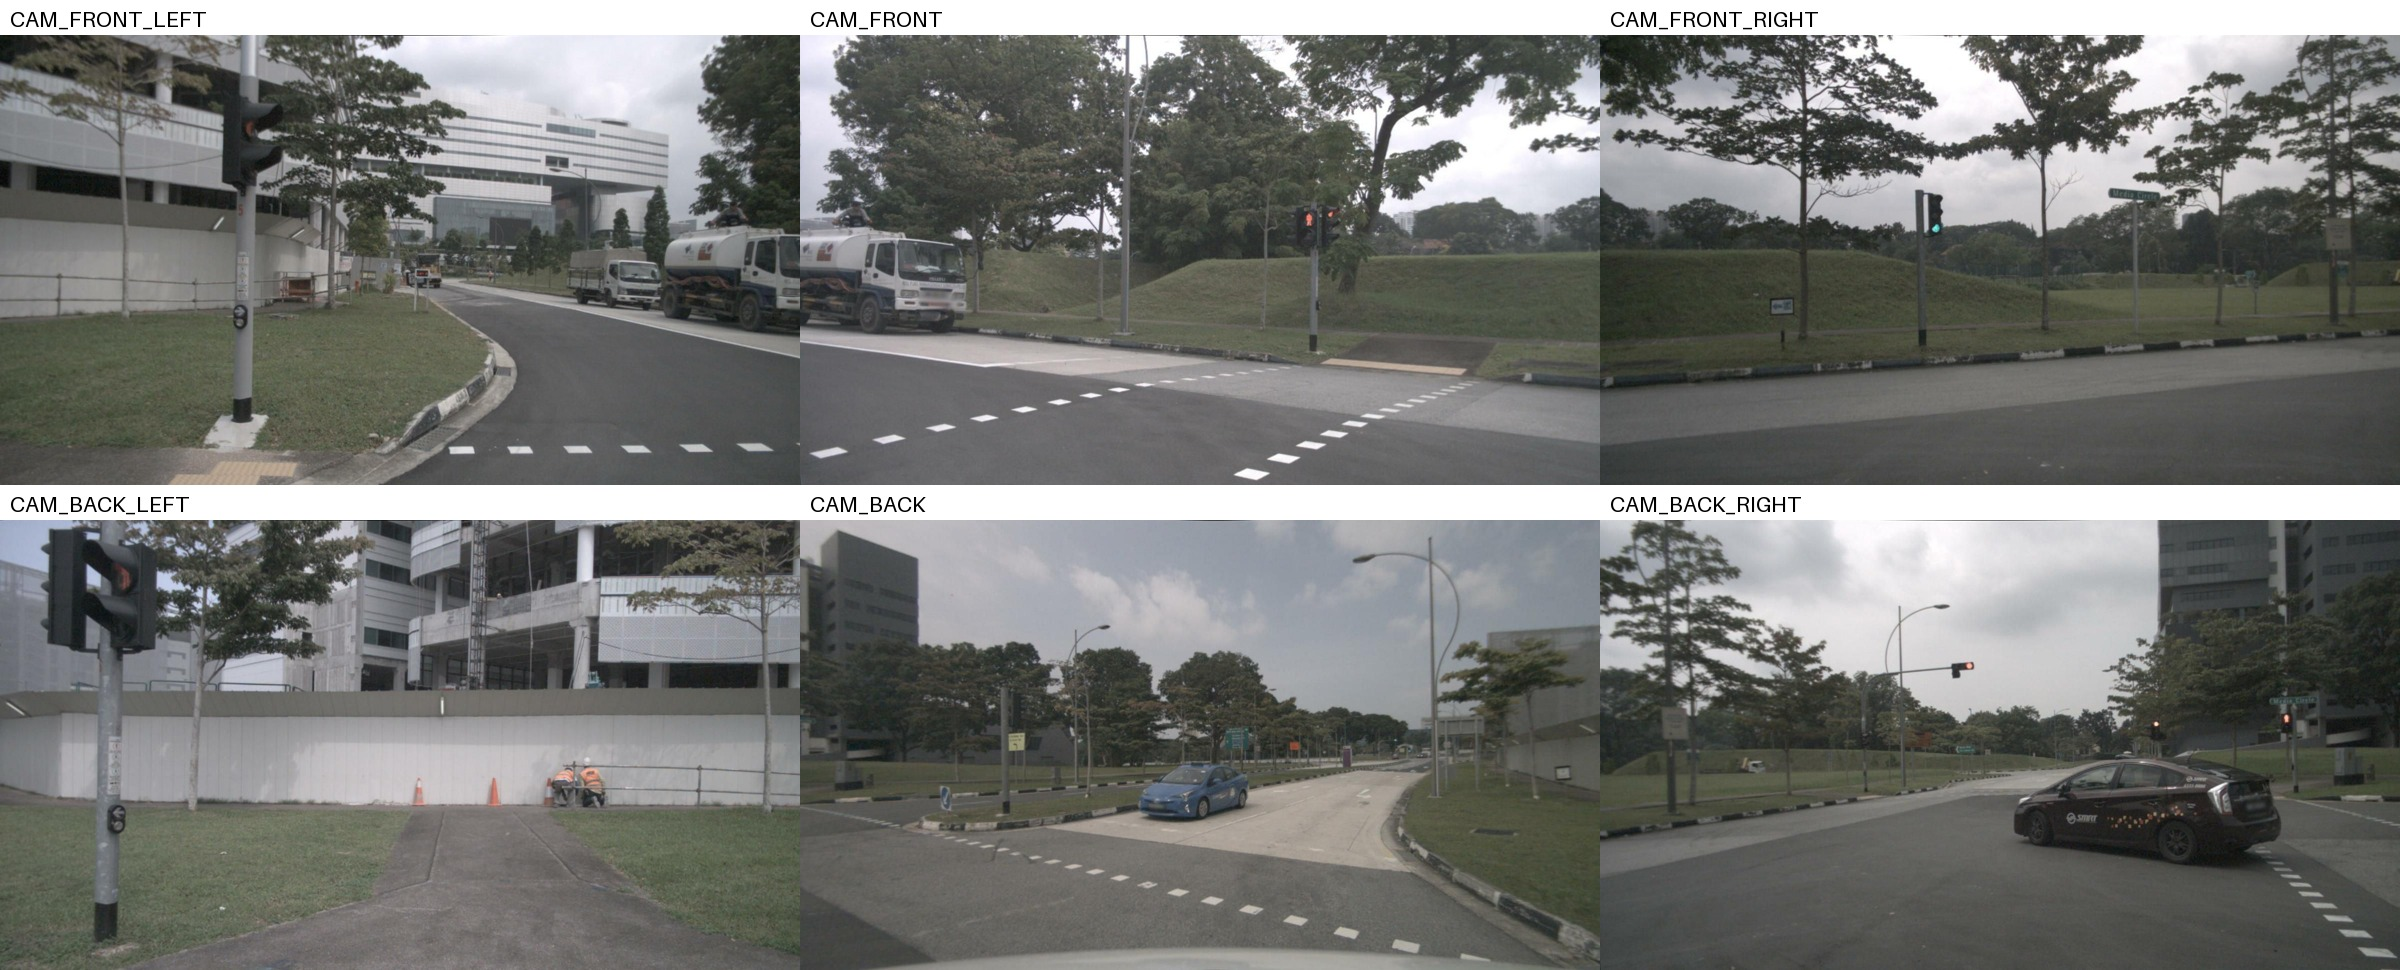
\includegraphics[width=\linewidth]{../../nuscenes_devkit/runs/20260923_133030_devkit_sample/camera_mosaic.jpg}
  \caption{同一 sample 的六路相机图像}
  \label{fig:camera-mosaic}
\end{figure}
\FloatBarrier

\subsection{相机标注与 LiDAR 点云显示}

同一脚本调用 DevKit 的 \texttt{render\_sample\_data()} 绘制前视相机和 LiDAR。图像显示
三维标注框，LiDAR 俯视图显示点云和目标框。课程数据没有 sweeps，因此设置
\texttt{nsweeps=1}。

\begin{figure}[htbp]
  \centering
  \begin{subfigure}[t]{0.48\linewidth}
    \centering
    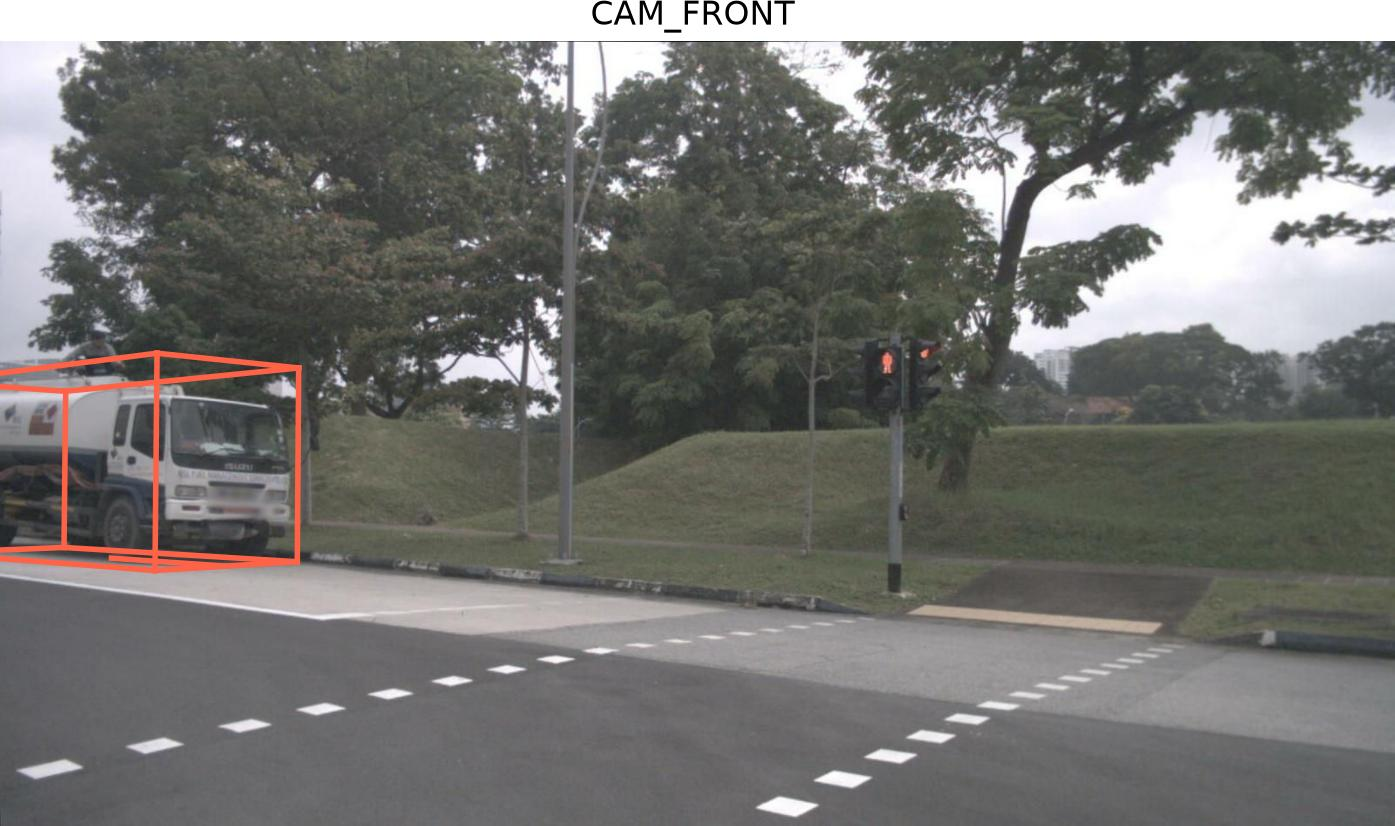
\includegraphics[width=\linewidth]{../../nuscenes_devkit/runs/20260923_133030_devkit_sample/cam_front_boxes.jpg}
    \caption{前视相机及三维标注框}
  \end{subfigure}
  \hfill
  \begin{subfigure}[t]{0.48\linewidth}
    \centering
    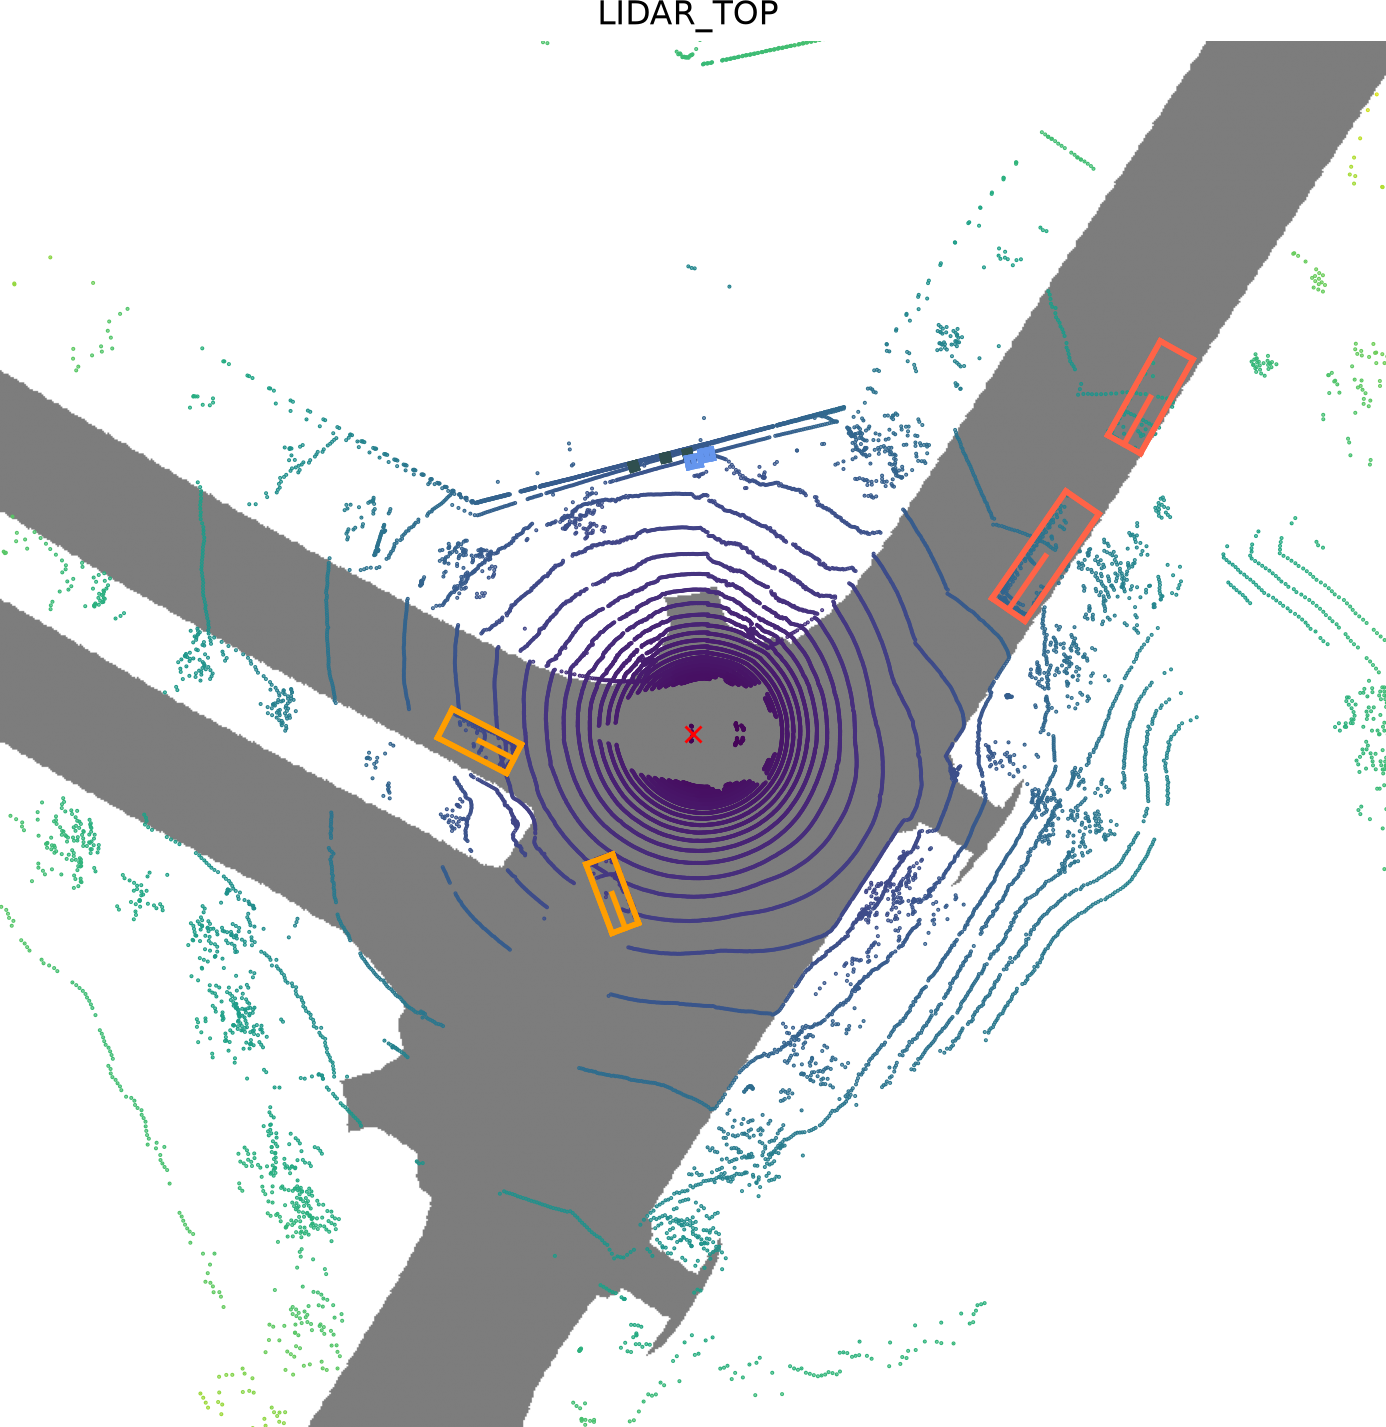
\includegraphics[width=\linewidth]{../../nuscenes_devkit/runs/20260923_133030_devkit_sample/lidar_top.png}
    \caption{LIDAR\_TOP 俯视图}
  \end{subfigure}
  \caption{DevKit 对相机和 LiDAR 数据的显示结果}
  \label{fig:devkit-render}
\end{figure}
\FloatBarrier

图~\ref{fig:devkit-render} 中，前视画面的三维框落在左侧卡车上，LiDAR 俯视图中的目标框
也贴合局部点云。

\section{多传感器坐标转换与可视化}

\subsection{坐标系与变换链}

nuScenes 的三维目标标注位于全局坐标系，相机、LiDAR 和 Radar 数据分别位于各自传感器坐标系。
\texttt{calibrated\_sensor} 给出 Sensor 与 Ego 之间的旋转和平移，\texttt{ego\_pose}
给出 Ego 与 Global 之间的关系。将 LiDAR 或 Radar 点投影到相机时，需要依次执行

\begin{equation}
  \text{Point Sensor} \rightarrow \text{Sensor Ego} \rightarrow \text{Global}
  \rightarrow \text{Camera Ego} \rightarrow \text{Camera Sensor}.
\end{equation}

得到相机坐标 $(X_c,Y_c,Z_c)$ 后，用相机内参矩阵 $\mathbf{K}$ 投影到像素平面：

\begin{equation}
  \lambda
  \begin{bmatrix} u \\ v \\ 1 \end{bmatrix}
  =
  \mathbf{K}
  \begin{bmatrix} X_c \\ Y_c \\ Z_c \end{bmatrix}.
\end{equation}

我比较了几个 scene 的画面，选用目标较清楚的 scene-0240。下面的叠加图和框转换图
由我运行 \path{nuscenes_devkit/project_lidar_camera.py} 生成。

\subsection{LiDAR 与 Radar 点云投影到相机}

\path{nuscenes_devkit/project_lidar_camera.py} 从同一 sample 取出 LIDAR\_TOP、RADAR\_FRONT 和
CAM\_FRONT 的 token，再调用 DevKit 完成投影。我在脚本中将 LiDAR 点按深度着色，Radar
点画成黄色，保存叠加图。关键代码是：

\begin{minted}{python}
lidar_token = sample["data"]["LIDAR_TOP"]
radar_token = sample["data"]["RADAR_FRONT"]
camera_token = sample["data"]["CAM_FRONT"]
lidar_count = save_pointcloud_projection(
    nusc, lidar_token, camera_token, output_dir / "lidar_on_camera.jpg", "LIDAR_TOP"
)
radar_count = save_pointcloud_projection(
    nusc, radar_token, camera_token, output_dir / "radar_on_camera.jpg", "RADAR_FRONT"
)
\end{minted}

scene-0240 中有 2,983 个 LiDAR 点落入前视图像。图~\ref{fig:lidar-camera} 用颜色表示
深度，车辆和道路上都能看到点云。

\begin{figure}[htbp]
  \centering
  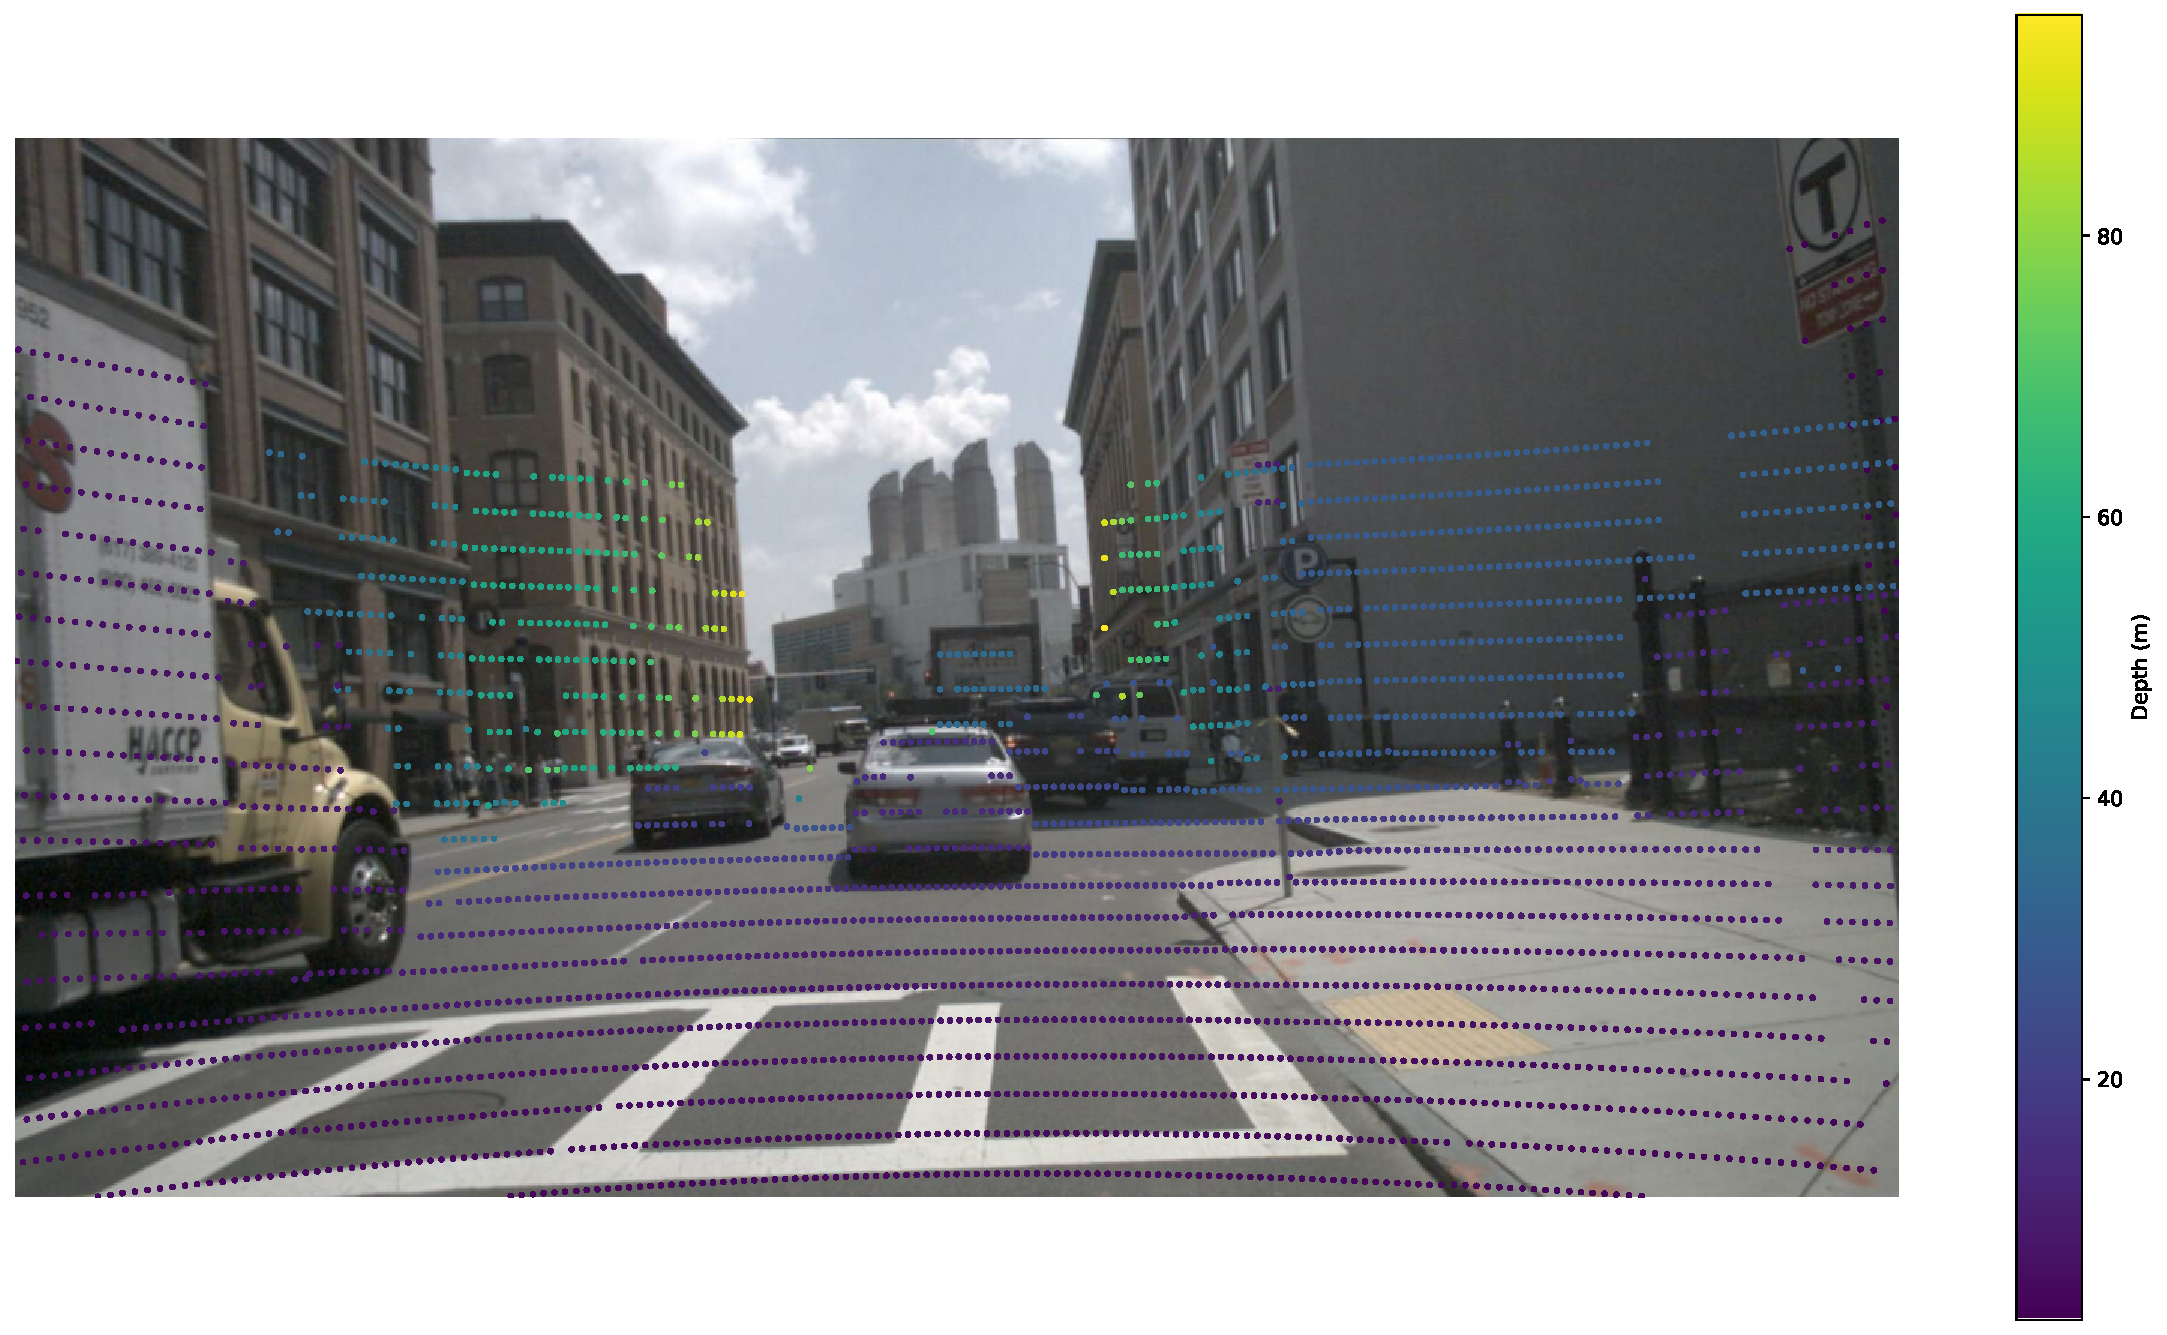
\includegraphics[width=0.94\linewidth]{../../nuscenes_devkit/runs/20260923_133749_lidar_camera/lidar_on_camera.pdf}
  \caption{LIDAR\_TOP 点云投影到 CAM\_FRONT，颜色表示深度}
  \label{fig:lidar-camera}
\end{figure}
\FloatBarrier

同一帧有 48 个 Radar 点落入前视图像，主要分布在前方车辆和路侧附近，明显比 LiDAR
稀疏，见图~\ref{fig:radar-camera}。

\begin{figure}[htbp]
  \centering
  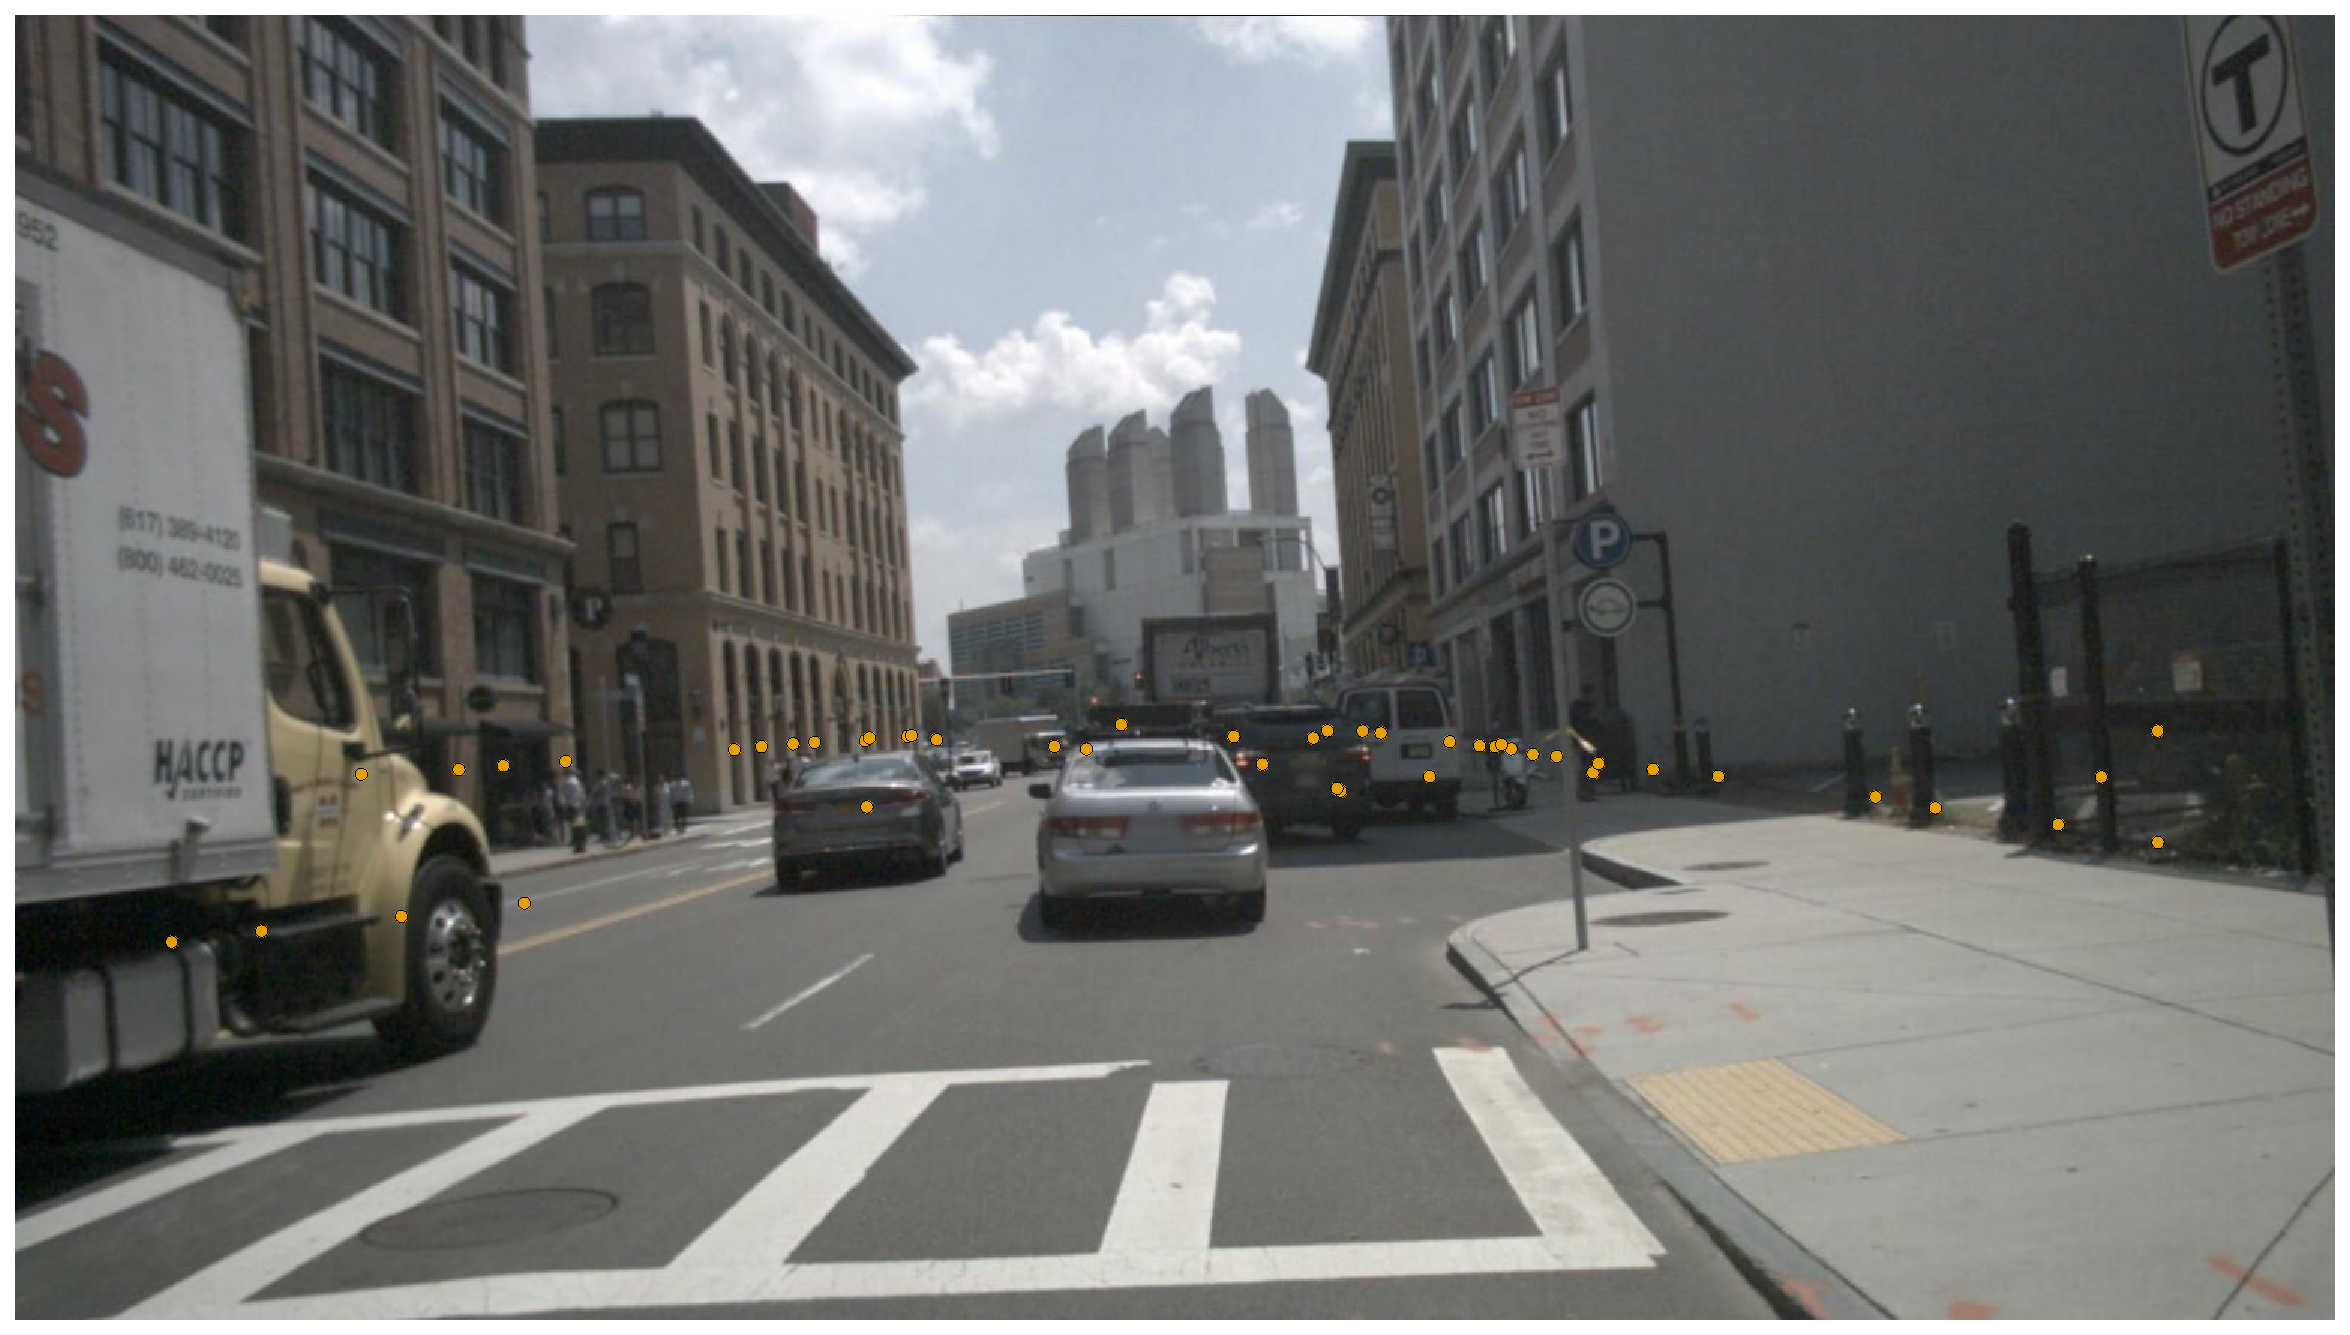
\includegraphics[width=0.94\linewidth]{../../nuscenes_devkit/runs/20260923_133749_lidar_camera/radar_on_camera.pdf}
  \caption{RADAR\_FRONT 点云投影到 CAM\_FRONT，黄色圆点为 Radar 回波}
  \label{fig:radar-camera}
\end{figure}
\FloatBarrier

\subsection{三维标注框转换为二维框}

在同一个 \path{nuscenes_devkit/project_lidar_camera.py} 中，我用 DevKit 取出相机视角下的三维框，
调用课程转换代码的 \texttt{project\_box()} 得到二维框，再把框画到图像上：

\begin{minted}{python}
image_path, boxes, intrinsic = nusc.get_sample_data(
    camera_token, box_vis_level=BoxVisibility.ANY
)
intrinsic_array = np.asarray(intrinsic)
config = FilterConfig()
for box in boxes:
    bbox = project_box(box, intrinsic_array, (width, height), config)
    if bbox is not None:
        draw.rectangle(bbox, outline="red", width=4)
\end{minted}

\begin{figure}[htbp]
  \centering
  \begin{subfigure}[t]{0.48\linewidth}
    \centering
    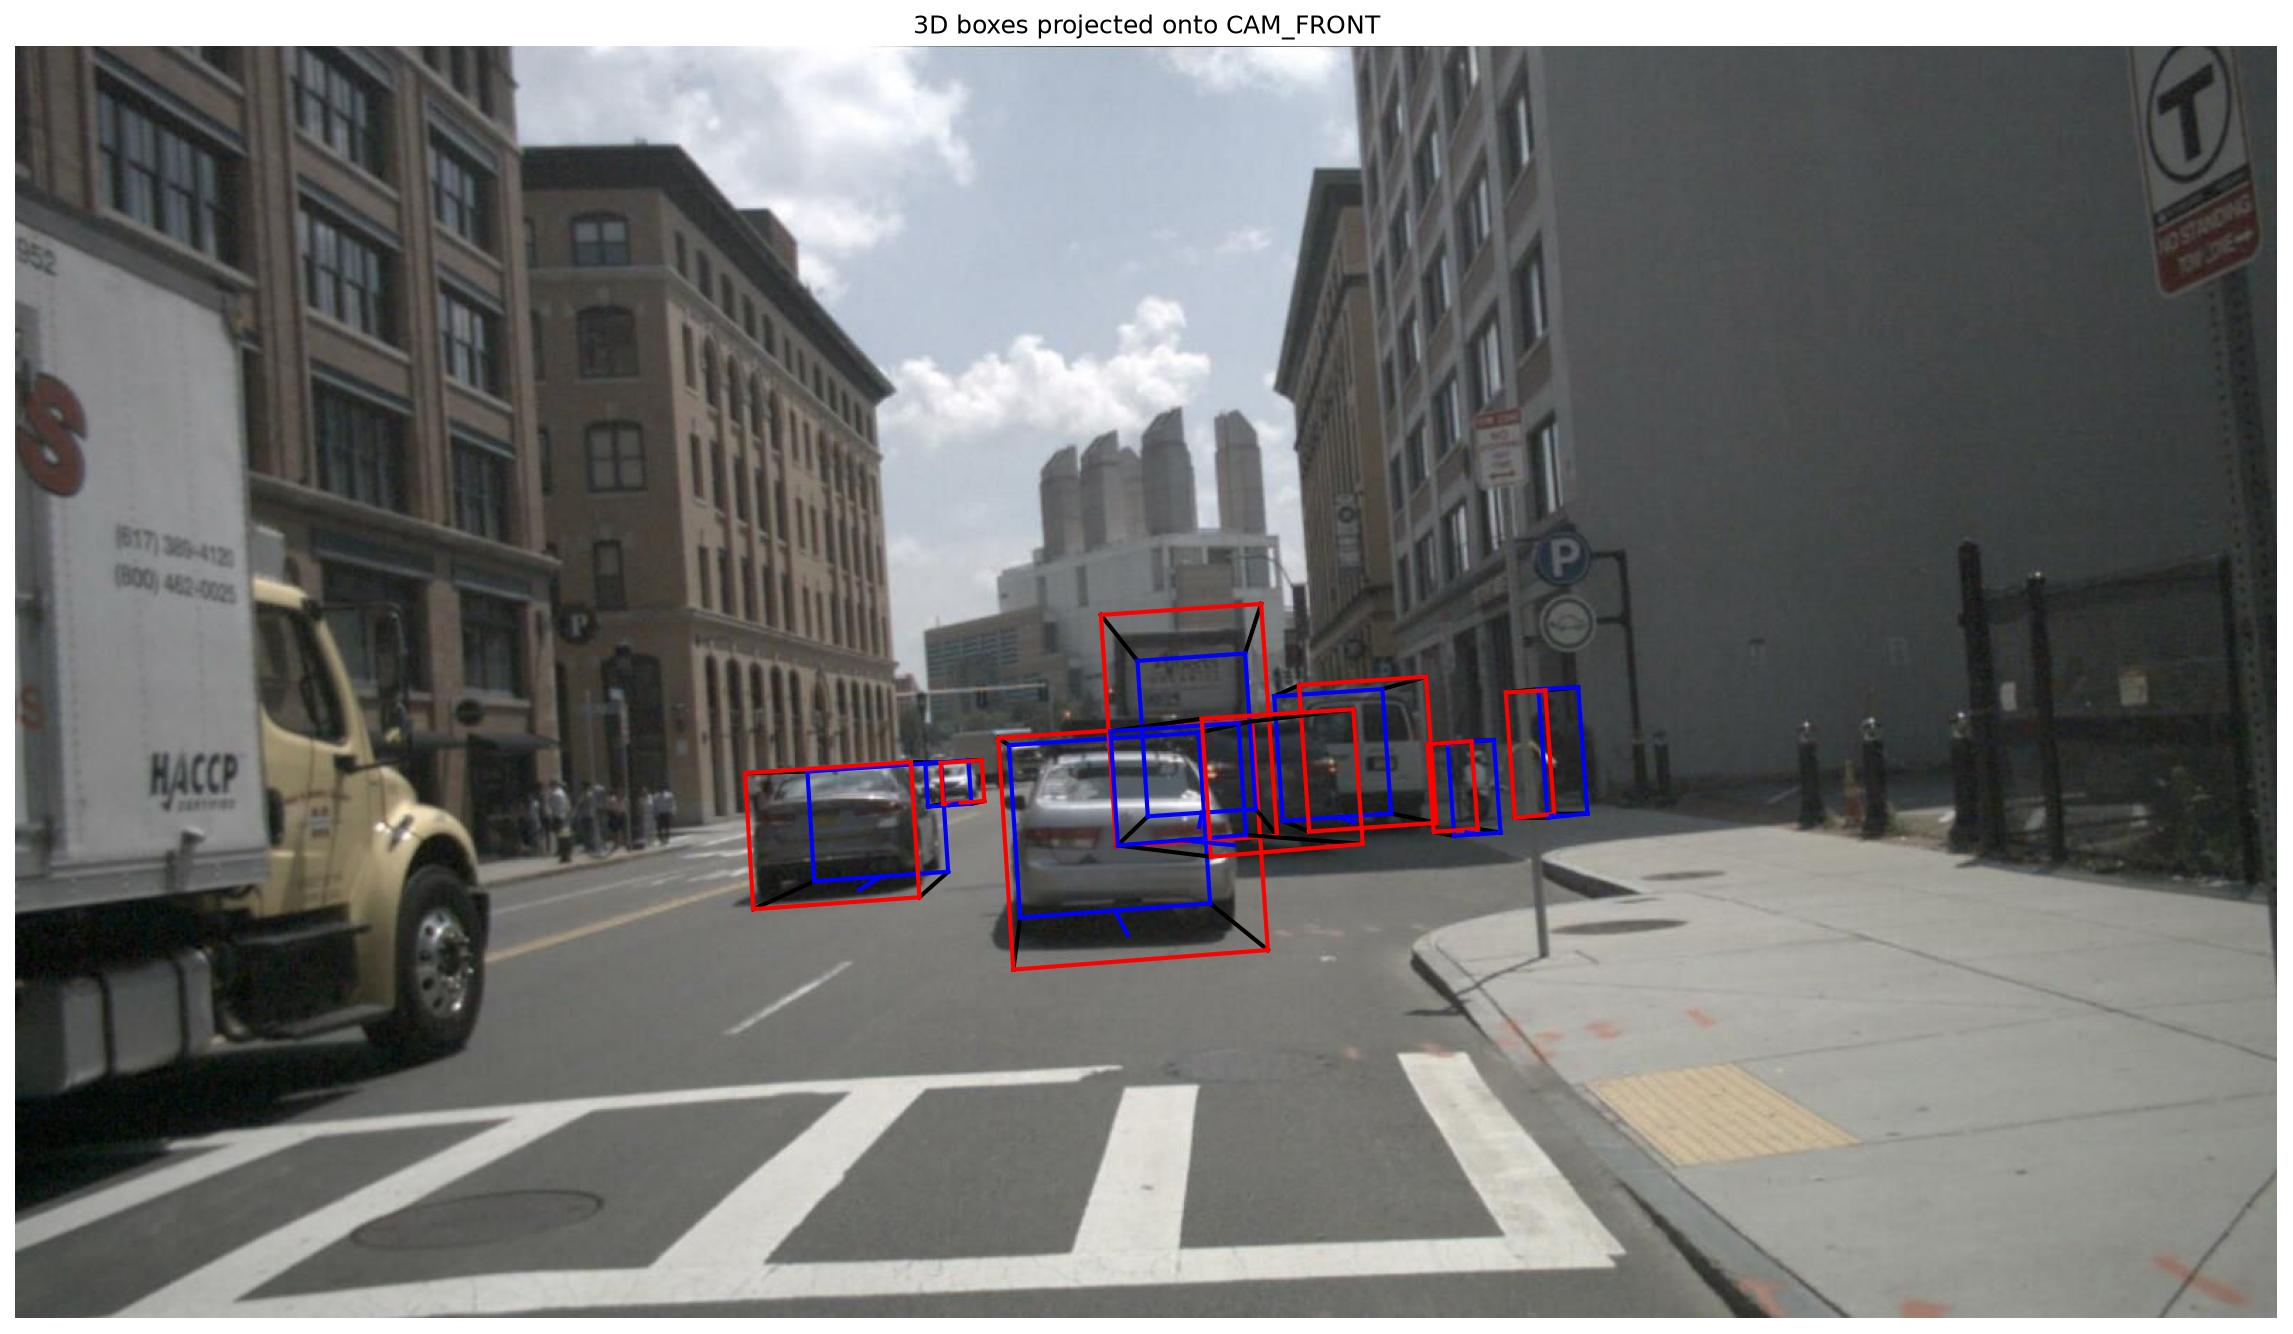
\includegraphics[width=\linewidth]{../../nuscenes_devkit/runs/20260923_133749_lidar_camera/boxes_3d_on_camera.jpg}
    \caption{相机坐标系中的三维框投影}
  \end{subfigure}
  \hfill
  \begin{subfigure}[t]{0.48\linewidth}
    \centering
    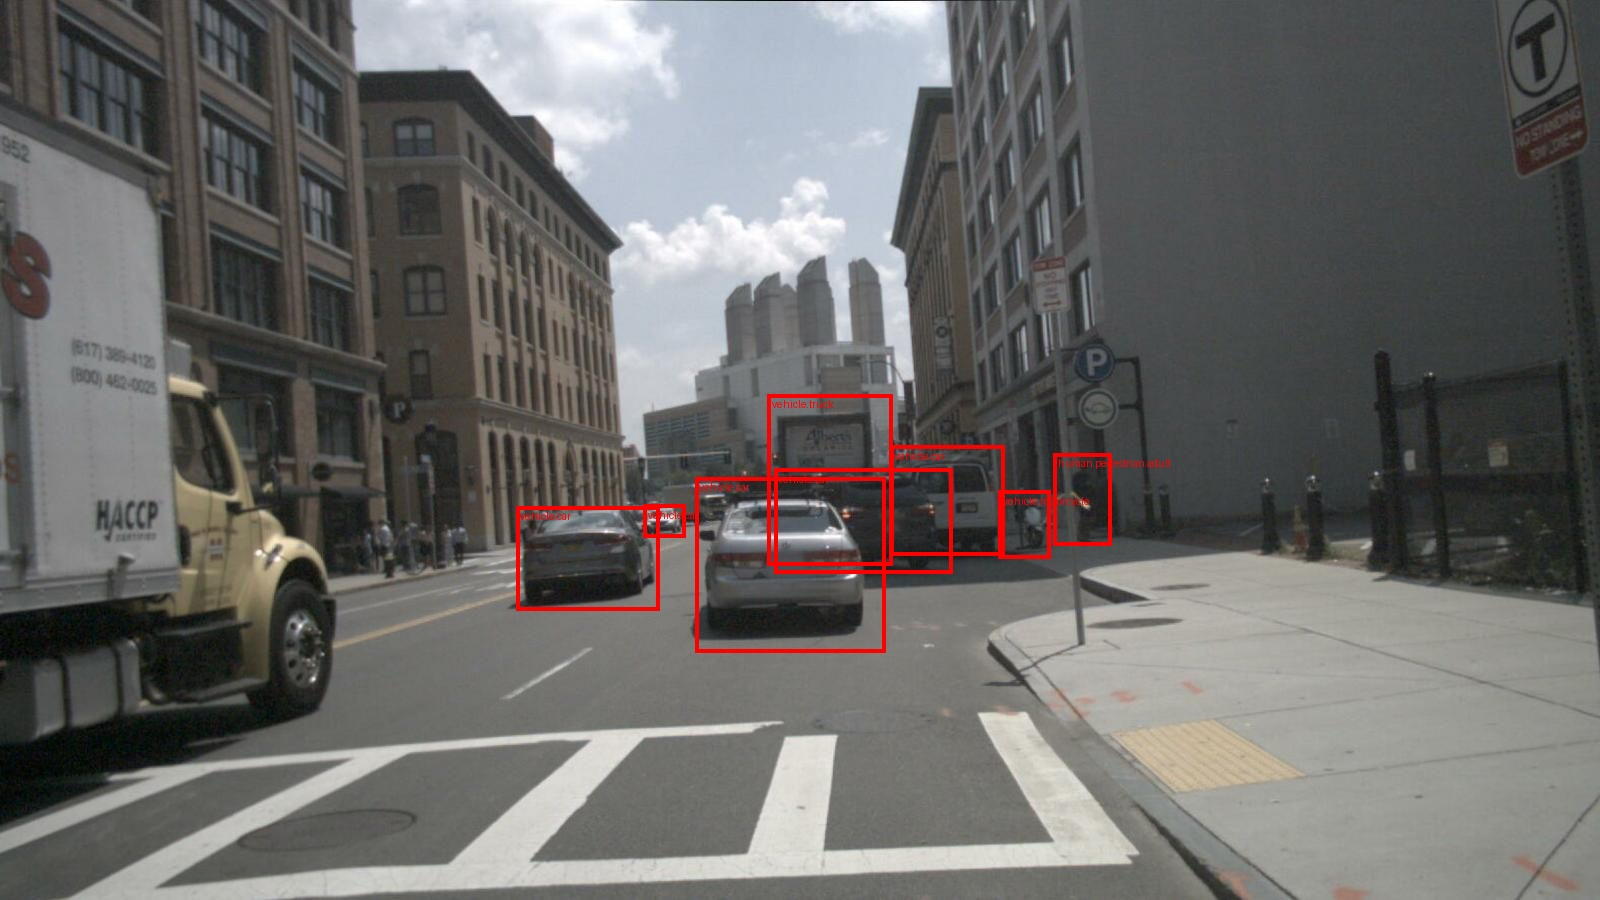
\includegraphics[width=\linewidth]{../../nuscenes_devkit/runs/20260923_133749_lidar_camera/boxes_2d_on_camera.jpg}
    \caption{三维角点生成的二维矩形框}
  \end{subfigure}
  \caption{同一帧三维框与二维包围框的转换结果}
  \label{fig:box-projection}
\end{figure}
\FloatBarrier

scene-0240 的这帧有 8 个三维框，转换后得到 8 个二维框，覆盖了图中的车辆、卡车和行人。

\section{nuScenes 到 YOLO 的数据格式转换}

\subsection{类别映射与标签格式}

课程转换程序将 nuScenes 的细分类别归并为 10 类：car、truck、bus、
trailer、construction\_vehicle、pedestrian、motorcycle、bicycle、traffic\_cone 和 barrier。

投影得到像素坐标 $(x_1,y_1,x_2,y_2)$ 后，YOLO 标签使用归一化中心点和宽高：

\begin{align}
  x_c &= \frac{x_1+x_2}{2W}, & y_c &= \frac{y_1+y_2}{2H}, \\
  w &= \frac{x_2-x_1}{W}, & h &= \frac{y_2-y_1}{H},
\end{align}

其中 $W$ 和 $H$ 为图像宽高。每行标签写为
\texttt{class\_id x\_center y\_center width height}，各坐标位于 $[0,1]$ 范围。

\subsection{目标筛选与数据划分}

课程数据使用前视相机的日间图像。转换程序保留可见比例约 60\% 以上、位于图像内且框足够大
的目标；车辆每移动至少 1 m 才保留下一帧。

每个地区按 scene 划分训练、验证和测试集，比例约为 7:1:2。

老师已经提供了转换后的数据。我对四个地区分别运行课程提供的
\path{nuscenes_yolo_converter/validate.py}：
21,502 张图像都有对应标签，128,712 个框
没有格式或坐标错误；还抽取图片查看了框的位置。

\section{YOLO11n 训练过程}

\subsection{模型与训练设置}

我运行 \path{yolo_workflow/train.sh}，由它调用老师提供的 \path{yolo_workflow/train.py}，使用
YOLO11n~\cite{ultralytics} 的 COCO 预训练权重 \texttt{yolo11n.pt} 训练 10 类目标。

训练使用 One-North 数据集，参数见表~\ref{tab:training-config}。

\begin{table}[htbp]
  \centering
  \caption{YOLO11n 正式训练配置}
  \label{tab:training-config}
  \begin{tabular}{ll}
    \toprule
    参数 & 设置 \\
    \midrule
    初始权重 & YOLO11n COCO 预训练权重 \\
    训练地区 & Singapore One-North \\
    Epochs & 50 \\
    Batch size & 16 \\
    输入尺寸 & $640\times640$ \\
    DataLoader workers & 16 \\
    设备 & CUDA:0 \\
    优化器 & Ultralytics auto \\
    AMP & 开启 \\
    \bottomrule
  \end{tabular}
\end{table}

训练耗时约 21 分钟，每轮的损失和指标保存在 \texttt{results.csv} 中。

\subsection{损失与验证指标}

图~\ref{fig:training-curves} 展示 50 轮训练曲线，表~\ref{tab:training-log} 摘出三轮日志。
训练 box loss 持续下降，验证 box loss 在中后期变化较小。

\begin{figure}[htbp]
  \centering
  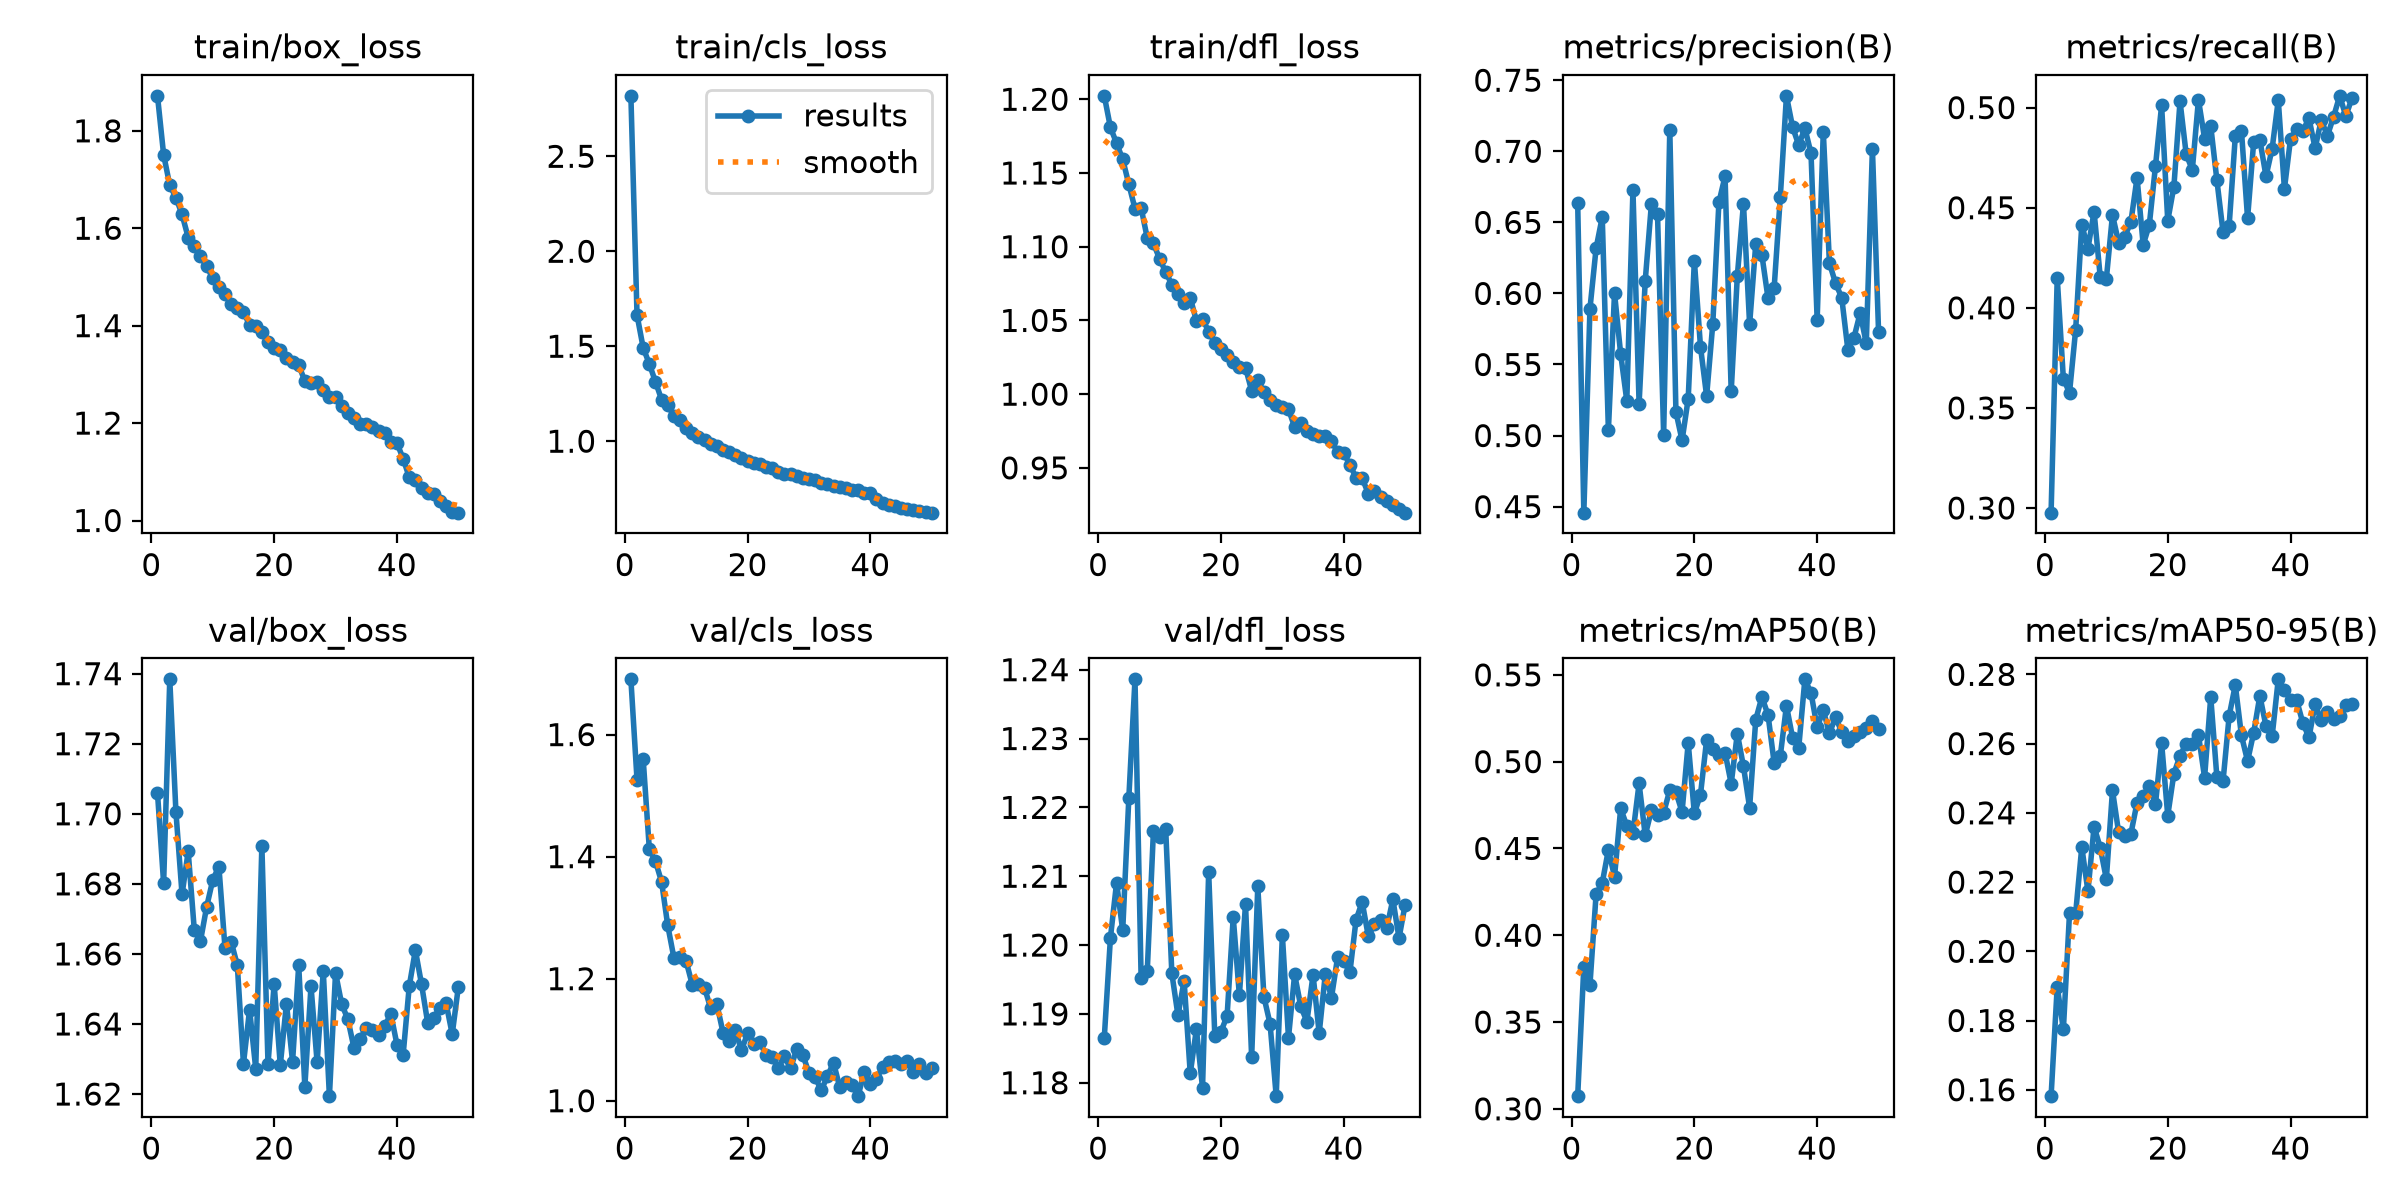
\includegraphics[width=\linewidth]{../../yolo_workflow/runs/checkpoints/20260916_092702_yolo11n_onenorth/results.png}
  \caption{YOLO11n 的训练损失和验证指标曲线}
  \label{fig:training-curves}
\end{figure}
\FloatBarrier

\begin{table}[htbp]
  \centering
  \caption{训练日志中的代表性轮次}
  \label{tab:training-log}
  \begin{tabular}{rrrr}
    \toprule
    Epoch & Train box loss & Val box loss & mAP@0.5:0.95 \\
    \midrule
    1 & 1.872 & 1.706 & 0.158 \\
    38 & 1.179 & 1.639 & 0.279 \\
    50 & 1.016 & 1.651 & 0.271 \\
    \bottomrule
  \end{tabular}
\end{table}
\FloatBarrier

第 38 轮的 mAP@0.5:0.95 最高，为 0.279。训练完成 50 轮后，我用第 38 轮保存的
\texttt{best.pt} 进行测试。

\section{模型测试与结果分析}

\subsection{独立测试集结果}

我运行 \path{yolo_workflow/evaluate.sh}，调用老师提供的 \path{yolo_workflow/evaluate.py} 加载
\texttt{best.pt}，评估 One-North 的 1,015 张测试图像。
结果见表~\ref{tab:test-results}，测试集与验证集的 mAP@0.5:0.95 接近。

\begin{table}[htbp]
  \centering
  \caption{One-North 验证集与测试集结果}
  \label{tab:test-results}
  \begin{tabular}{lrrrr}
    \toprule
    数据划分 & Precision & Recall & mAP@0.5 & mAP@0.5:0.95 \\
    \midrule
    Validation（第 38 轮） & 0.716 & 0.504 & 0.547 & 0.279 \\
    Test & 0.686 & 0.505 & 0.548 & 0.288 \\
    \bottomrule
  \end{tabular}
\end{table}

测试集 Recall 为 0.505。查看预测图片时，我发现远处的小行人和自行车有漏检。

\subsection{类别表现与混淆矩阵}

归一化混淆矩阵见图~\ref{fig:confusion}。car、truck 和 bus 的对角元素约为 0.83、
0.79 和 0.82；bicycle、traffic cone 和 barrier 的漏检更多。

\begin{figure}[htbp]
  \centering
  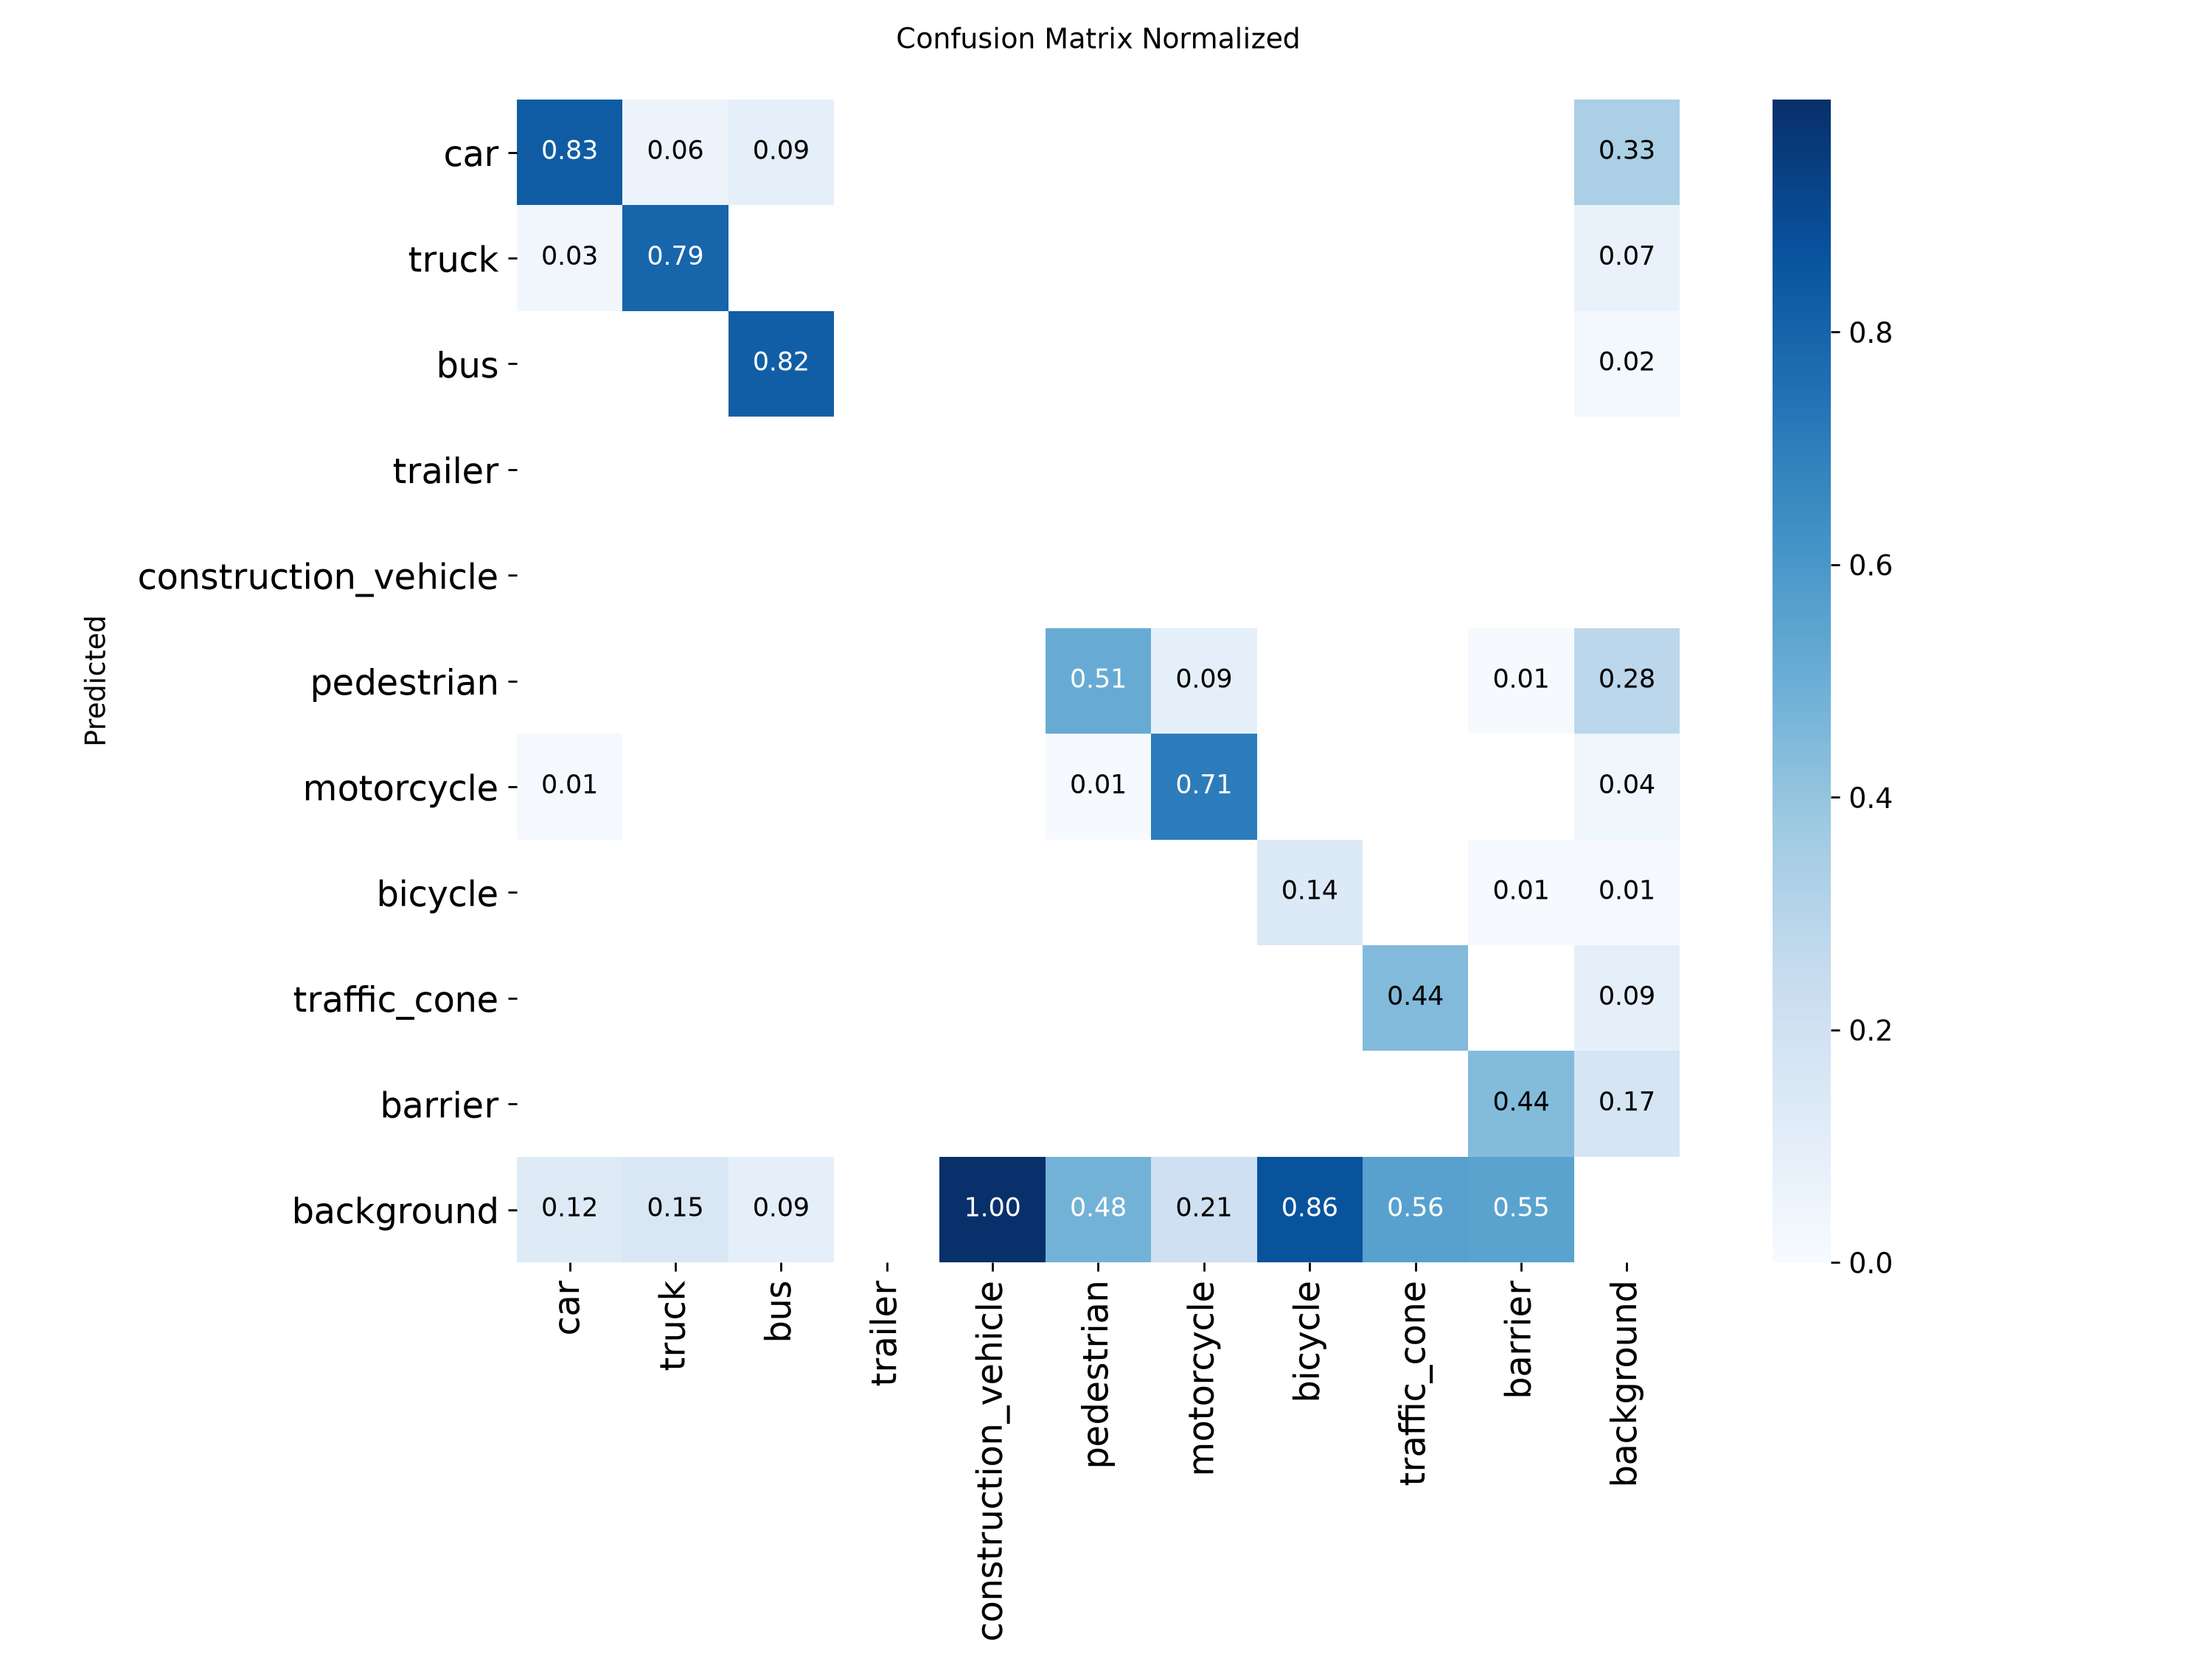
\includegraphics[width=0.78\linewidth]{../../yolo_workflow/runs/checkpoints/20260916_092702_yolo11n_onenorth/confusion_matrix_normalized.png}
  \caption{验证集归一化混淆矩阵}
  \label{fig:confusion}
\end{figure}
\FloatBarrier

模型对常见车辆的识别更稳定，小目标漏检较多。

\subsection{预测案例}

\texttt{evaluate.py} 在测试时生成了真实标签与预测对比图。图~\ref{fig:test-comparison}
中，道路两侧的车辆和部分行人被检出，较小、较远的目标有些没有预测框。

\begin{figure}[htbp]
  \centering
  \begin{subfigure}[t]{0.48\linewidth}
    \centering
    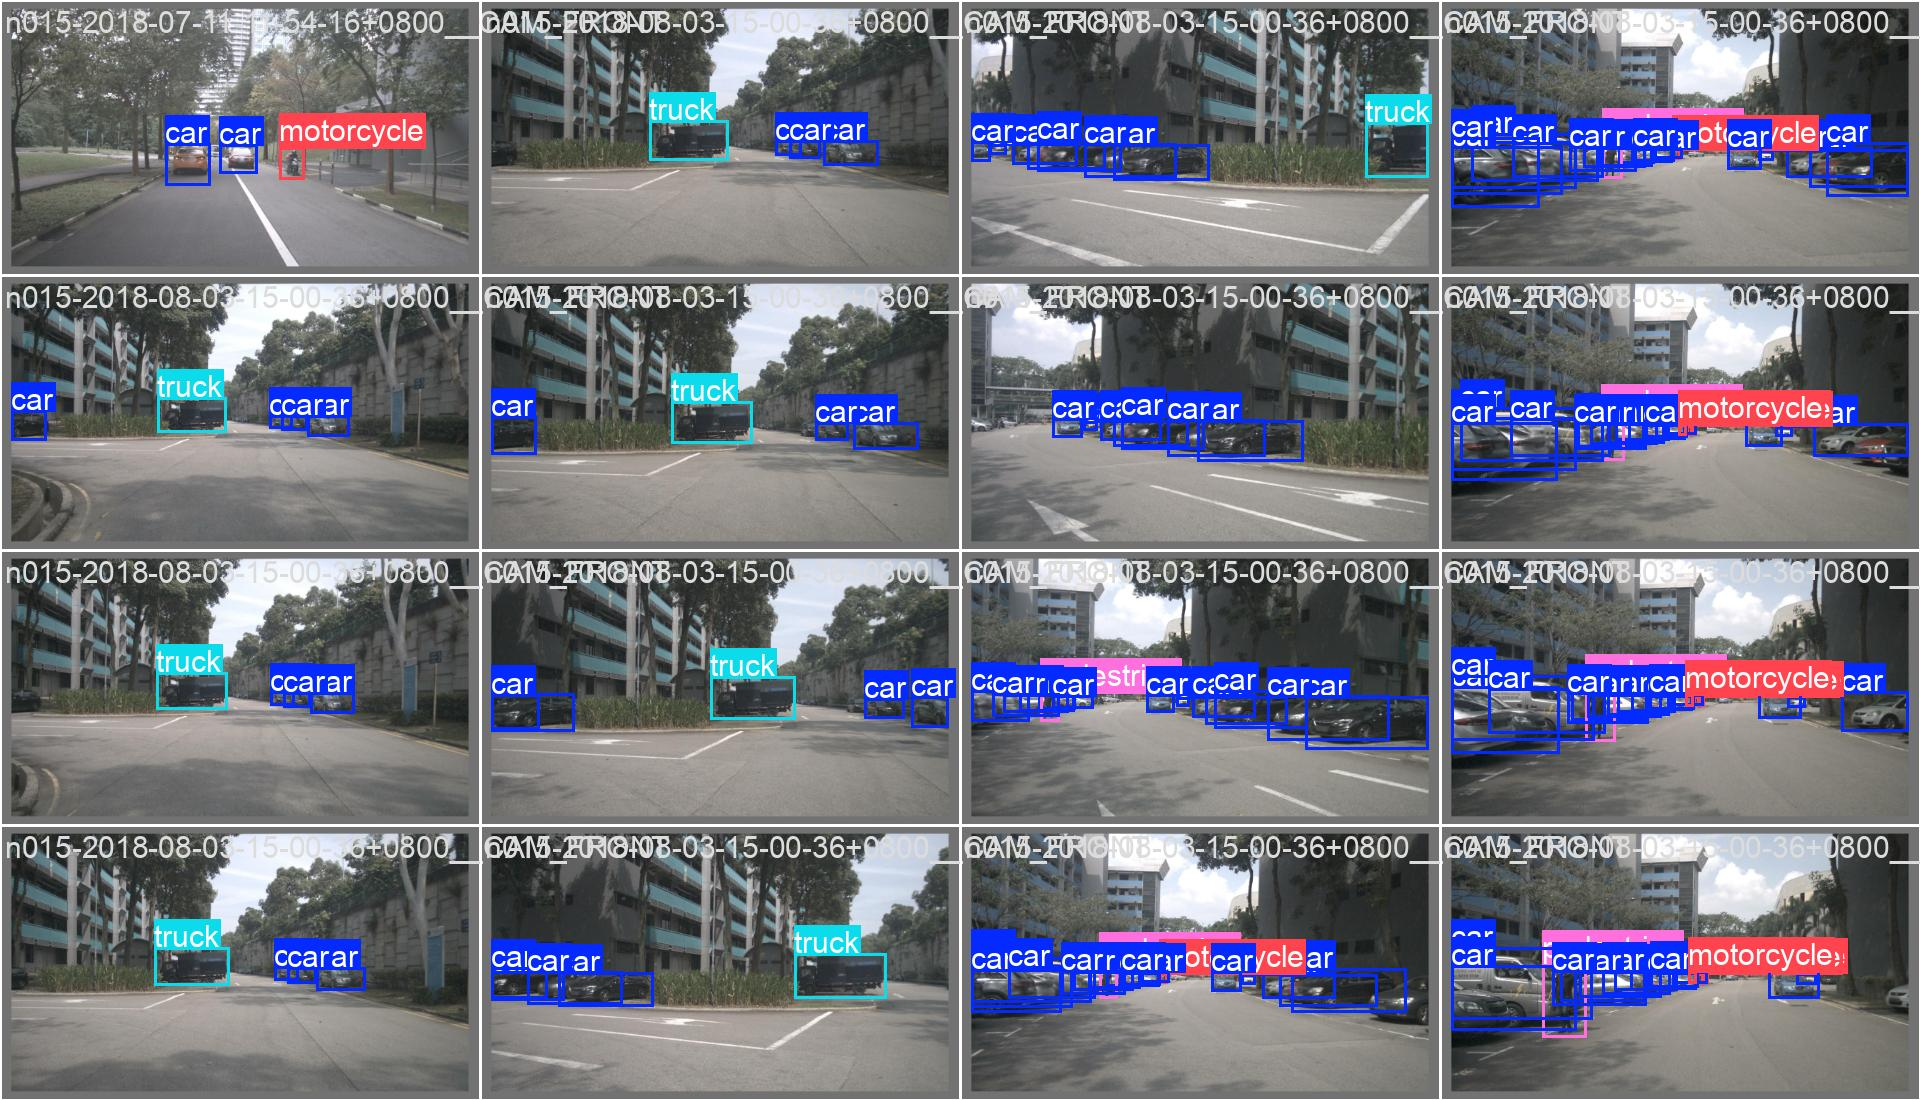
\includegraphics[width=\linewidth]{../../yolo_workflow/runs/evaluation/20260916_095228_yolo11n_onenorth_test_val_test/val_batch0_labels.jpg}
    \caption{测试图像真实标签}
  \end{subfigure}
  \hfill
  \begin{subfigure}[t]{0.48\linewidth}
    \centering
    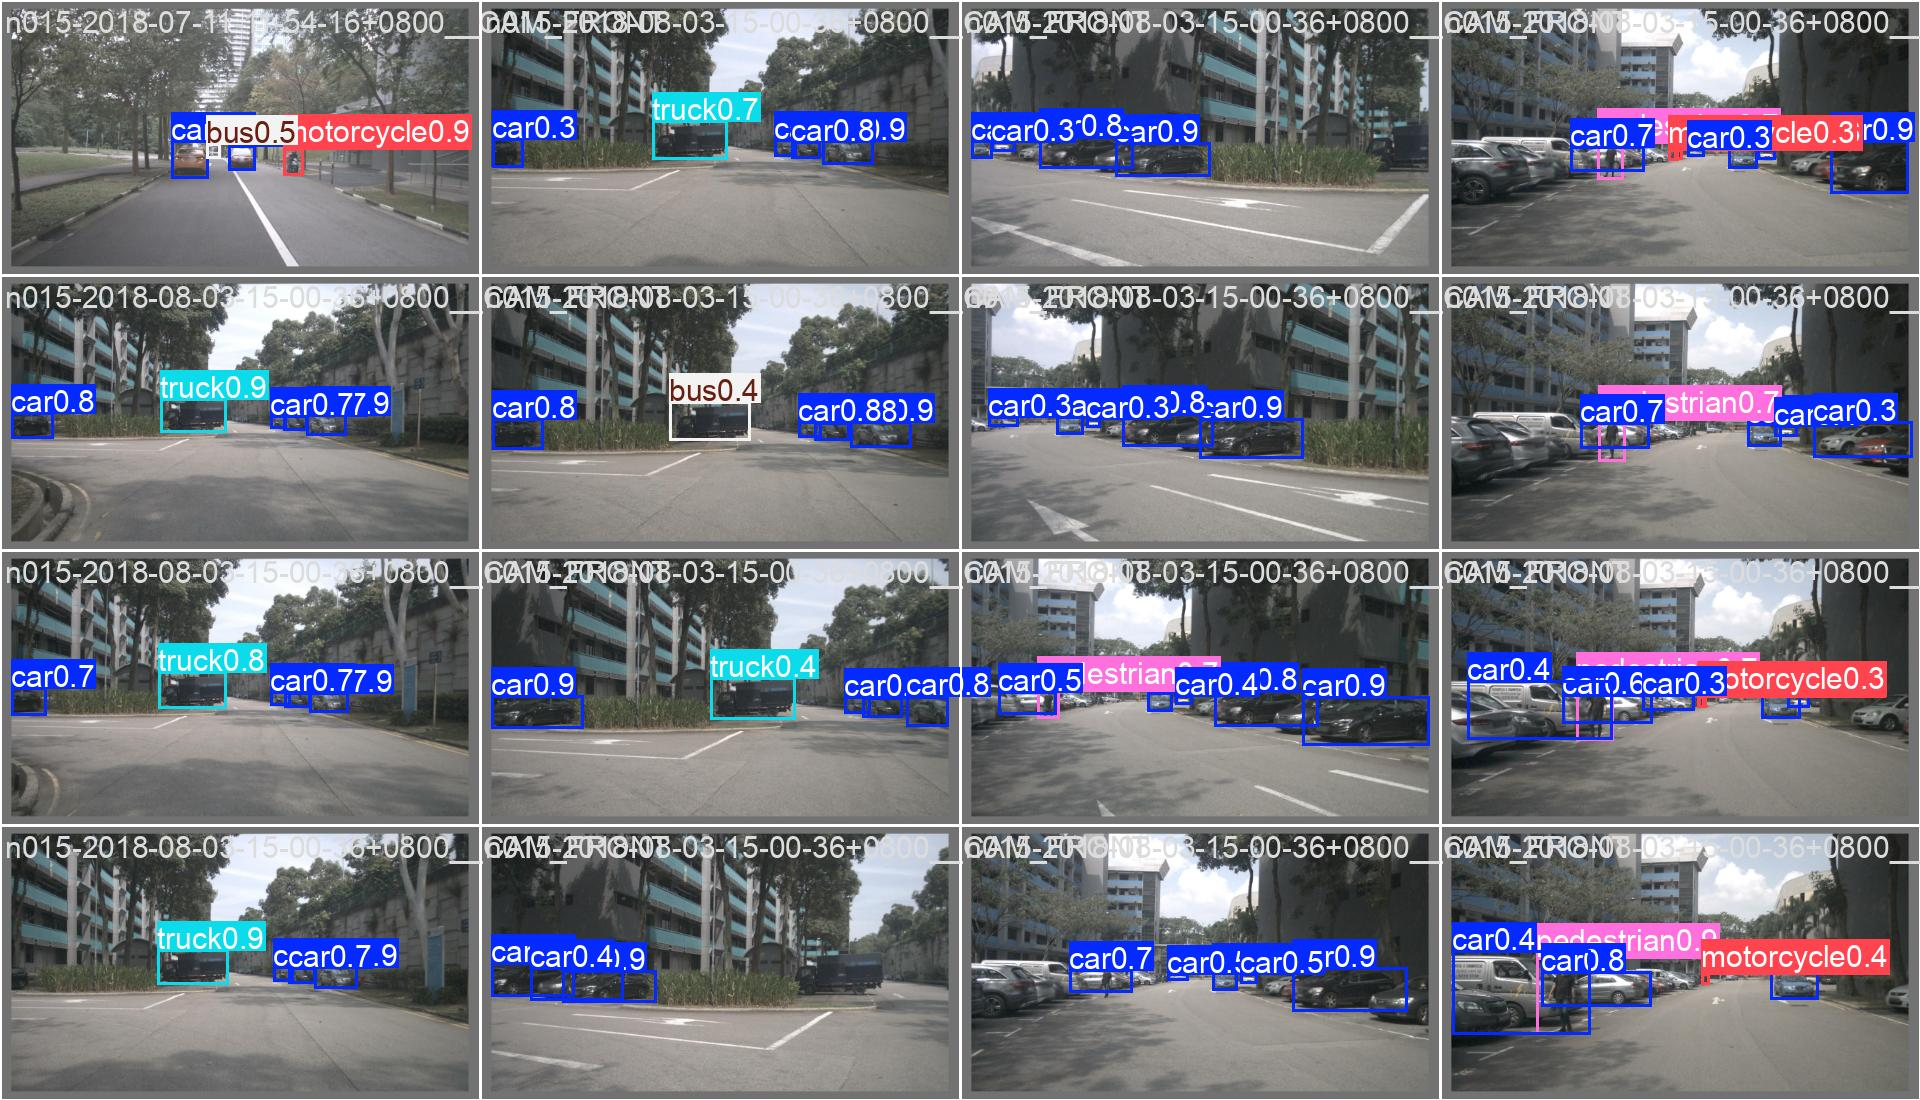
\includegraphics[width=\linewidth]{../../yolo_workflow/runs/evaluation/20260916_095228_yolo11n_onenorth_test_val_test/val_batch0_pred.jpg}
    \caption{YOLO11n 预测结果}
  \end{subfigure}
  \caption{One-North 测试集真实标签与预测结果对比}
  \label{fig:test-comparison}
\end{figure}
\FloatBarrier

\clearpage
\section{跨地区泛化实验}

\subsection{实验设计}

完成 One-North 测试后，我写了跨地区评估脚本
\path{yolo_workflow/evaluate_cross_location.py}，通过
\path{yolo_workflow/evaluate_cross_location.sh} 运行。它用同一份 \texttt{best.pt} 依次测试
四个地区，汇总指标并绘制图~\ref{fig:cross-location}。其中的循环是：

\begin{minted}{python}
model = YOLO(str(model_path))
for location in LOCATIONS:
    data_yaml = datasets_root / location / "data.yaml"
    metrics = model.val(
        data=str(data_yaml), split="test", imgsz=args.imgsz,
        batch=args.batch, device=args.device, workers=args.workers,
        conf=0.001, iou=0.7,
    )
    rows.append({
        "location": location,
        "images": sum(1 for path in (data_yaml.parent / "images/test").iterdir() if path.is_file()),
        "precision": float(metrics.box.mp),
        "recall": float(metrics.box.mr),
        "mAP50": float(metrics.box.map50),
        "mAP50-95": float(metrics.box.map),
    })
\end{minted}

\subsection{实验结果}

\begin{table}[htbp]
  \centering
  \caption{YOLO11n 跨地区测试结果}
  \label{tab:cross-location}
  \begin{tabular}{lrrrrr}
    \toprule
    测试地区 & 图像数 & Precision & Recall & mAP@0.5 & mAP@0.5:0.95 \\
    \midrule
    Boston Seaport & 2,709 & 0.389 & 0.195 & 0.156 & 0.071 \\
    Holland Village & 88 & 0.665 & 0.430 & 0.445 & 0.275 \\
    One-North & 1,015 & 0.686 & 0.505 & 0.548 & 0.288 \\
    Queenstown & 486 & 0.544 & 0.544 & 0.538 & 0.259 \\
    \bottomrule
  \end{tabular}
\end{table}

\begin{figure}[htbp]
  \centering
  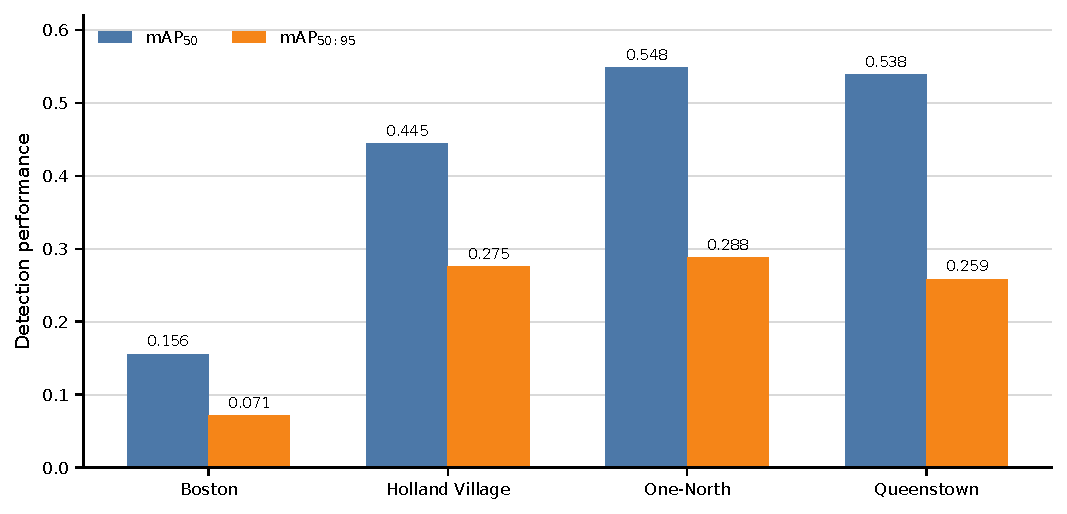
\includegraphics[width=0.92\linewidth]{../../yolo_workflow/runs/cross_location/20260922_174056_yolo11n_onenorth_cross_location/comparison.pdf}
  \caption{One-North 训练模型在四个地区测试集上的检测性能}
  \label{fig:cross-location}
\end{figure}
\FloatBarrier

三个新加坡地区的 mAP@0.5:0.95 在 0.259 至 0.288 之间；Holland Village 的测试集
只有 88 张图像。

Boston 的 mAP@0.5:0.95 为 0.071，Recall 为 0.195，漏检明显更多。查看图像时，我也
看到它的道路和建筑与新加坡地区不同。

\section{问题分析与实验总结}

\subsection{实验中遇到的问题}

数据保存在机械硬盘。Boston 测试时，Ultralytics 提示图像读取较慢。

训练数据中 construction\_vehicle、bicycle 等类别的数量较少；测试图像里也能看到这些
类别的漏检。

\subsection{实验总结}

这次实验完成了 nuScenes 数据读取、LiDAR 和 Radar 点云投影、三维框转二维框，以及
YOLO11n 的训练与测试。One-North 测试集的 mAP@0.5:0.95 为 0.288；换到 Boston 后降至
0.071。预测图中，远处小目标的漏检较明显。

\begin{thebibliography}{9}
  \bibitem{nuscenes}
  H. Caesar et al., ``nuScenes: A Multimodal Dataset for Autonomous Driving,''
  \textit{Proceedings of the IEEE/CVF Conference on Computer Vision and Pattern Recognition},
  2020, pp. 11621--11631.

  \bibitem{ultralytics}
  Ultralytics, ``Ultralytics YOLO Documentation,''
  \url{https://docs.ultralytics.com/}.

\end{thebibliography}

\end{document}
